\documentclass{article}

\usepackage{polski}
\usepackage[utf8]{inputenc}

\usepackage{fancyhdr} % Required for custom headers
\usepackage{lastpage} % Required to determine the last page for the footer
\usepackage{extramarks} % Required for headers and footers
\usepackage[usenames,dvipsnames]{color} % Required for custom colors
\usepackage{graphicx} % Required to insert images
\usepackage{listings} % Required for insertion of code
\usepackage{courier} % Required for the courier font
\usepackage{lipsum} 
\usepackage{amsfonts}
\usepackage{amsthm}
\usepackage{hyperref}
\usepackage{tikz}
\usepackage{amsmath}
\usepackage{pdfpages}
\usepackage{mathtools}
\usepackage{enumitem}

\usepackage{amsthm}
\usepackage{epigraph}

\DeclareUnicodeCharacter{00A0}{ }

\makeatletter
\newenvironment{chapquote}[2][2em]
  {\setlength{\@tempdima}{#1}%
   \def\chapquote@author{#2}%
   \parshape 1 \@tempdima \dimexpr\textwidth-2\@tempdima\relax%
   \itshape}
  {\par\normalfont\hfill--\ \chapquote@author\hspace*{\@tempdima}\par\bigskip}
\makeatother

\newtheorem{thm}{Twierdzenie}
\newtheorem{remark}{Uwaga}
\newtheorem{lemat}{Lemat}
\newtheorem{wniosek}{Wniosek}
\newtheorem{definicja}{Definicja}
\newtheorem{ciekawostka}{Ciekawostka}
\newtheorem{przyklad}{Przykład}
\newtheorem{fakt}{Fakt}



\newenvironment{prooff}{\paragraph{Dowód:}}{\hfill$\square$}
\newenvironment{rozw}{\paragraph{Rozwiązanie:}}{\hfill}


\usepackage{inconsolata} % very nice fixed-width font included with texlive-full
\usepackage[usenames,dvipsnames]{color} % more flexible names for syntax highlighting colors
\usepackage{listings}

\lstset{
basicstyle=\small\ttfamily, 
columns=fullflexible, % make sure to use fixed-width font, CM typewriter is NOT fixed width
numbers=left, 
numberstyle=\small\ttfamily\color{Gray},
stepnumber=1,              
numbersep=10pt, 
numberfirstline=true, 
numberblanklines=true, 
tabsize=4,
lineskip=-1.5pt,
extendedchars=true,
breaklines=true,        
keywordstyle=\color{Blue}\bfseries,
identifierstyle=, % using emph or index keywords
commentstyle=\sffamily\color{OliveGreen},
stringstyle=\color{Maroon},
showstringspaces=false,
showtabs=false,
upquote=false,
texcl=true, % interpret comments as LaTeX
    literate={á}{{\'a}}1 {ã}{{\~a}}1 {é}{{<}}1,
inputencoding=utf8
}

\lstdefinelanguage{julia}
{
  keywordsprefix=\@,
  morekeywords={
    exit,whos,edit,load,is,isa,isequal,typeof,tuple,ntuple,uid,hash,finalizer,convert,promote,
    subtype,typemin,typemax,realmin,realmax,sizeof,eps,promote_type,method_exists,applicable,
    invoke,dlopen,dlsym,system,error,throw,assert,new,Inf,Nan,pi,im,begin,while,for,in,return,
    break,continue,macro,quote,let,if,elseif,else,try,catch,end,bitstype,ccall,do,using,module,
    import,export,importall,baremodule,immutable,local,global,const,Bool,Int,Int8,Int16,Int32,
    Int64,Uint,Uint8,Uint16,Uint32,Uint64,Float32,Float64,Complex64,Complex128,Any,Nothing,None,
    function,type,typealias,abstract
  },
  sensitive=true,
  morecomment=[l]{\#},
  morestring=[b]',
  morestring=[b]" 
}

% Margins
\topmargin=-0.45in
\evensidemargin=0in
\oddsidemargin=0in
\textwidth=6.0in
\textheight=9.0in
\headsep=0.25in

\linespread{1.1} % Line spacing

% Set up the header and footer
\pagestyle{fancy}
\lhead{\hmwkAuthorName} % Top left header
\rhead{\firstxmark} % Top right header
\lfoot{\lastxmark} % Bottom left footer
\cfoot{} % Bottom center footer
\renewcommand\headrulewidth{0.4pt} % Size of the header rule
\renewcommand\footrulewidth{0.4pt} % Size of the footer rule

\setlength\parindent{0pt} % Removes all indentation from paragraphs
%----------------------------------------------------------------------------------------
%	DOCUMENT STRUCTURE COMMANDS
%	Skip this unless you know what you're doing
%----------------------------------------------------------------------------------------

% Header and footer for when a page split occurs within a problem environment
\newcommand{\enterProblemHeader}[1]{
\nobreak\extramarks{#1}{#1 continued on next page\ldots}\nobreak
\nobreak\extramarks{#1 (continued)}{#1 continued on next page\ldots}\nobreak
}

% Header and footer for when a page split occurs between problem environments
\newcommand{\exitProblemHeader}[1]{
\nobreak\extramarks{#1 (continued)}{#1 continued on next page\ldots}\nobreak
\nobreak\extramarks{#1}{}\nobreak
}

\setcounter{secnumdepth}{0} % Removes default section numbers
\newcounter{homeworkProblemCounter} % Creates a counter to keep track of the number of problems

\newcommand{\homeworkProblemName}{}
\newenvironment{homeworkProblem}[1][Zadanie \arabic{homeworkProblemCounter}]{ % Makes a new environment called homeworkProblem which takes 1 argument (custom name) but the default is "Problem #"
\stepcounter{homeworkProblemCounter} % Increase counter for number of problems
\renewcommand{\homeworkProblemName}{#1} % Assign \homeworkProblemName the name of the problem
\section{\homeworkProblemName} % Make a section in the document with the custom problem count
\enterProblemHeader{\homeworkProblemName} % Header and footer within the environment
}{
\exitProblemHeader{\homeworkProblemName} % Header and footer after the environment
}

\newcommand{\problemAnswer}[1]{ % Defines the problem answer command with the content as the only argument
\noindent\framebox[\columnwidth][c]{\begin{minipage}{0.98\columnwidth}#1\end{minipage}} % Makes the box around the problem answer and puts the content inside
}

\newcommand{\homeworkSectionName}{}
\newenvironment{homeworkSection}[1]{ % New environment for sections within homework problems, takes 1 argument - the name of the section
\renewcommand{\homeworkSectionName}{#1} % Assign \homeworkSectionName to the name of the section from the environment argument
\subsection{\homeworkSectionName} % Make a subsection with the custom name of the subsection
\enterProblemHeader{\homeworkProblemName\ [\homeworkSectionName]} % Header and footer within the environment
}{
\enterProblemHeader{\homeworkProblemName} % Header and footer after the environment
}

\usepackage{listings} % Required for inserting code snippets
\usepackage[usenames,dvipsnames]{color} % Required for specifying custom colors and referring to colors by name

\definecolor{DarkGreen}{rgb}{0.0,0.4,0.0} % Comment color
\definecolor{highlight}{RGB}{255,251,204} % Code highlight color

% Create a command to cleanly insert a snippet with the style above anywhere in the document
\newcommand{\insertcode}[2]{\begin{itemize}\item[]\lstinputlisting[caption=#2,label=#1,style=Style1]{#1}\end{itemize}} % The first argument is the script location/filename and the second is a caption for the listing

%----------------------------------------------------------------------------------------
%	NAME AND CLASS SECTION
%----------------------------------------------------------------------------------------

\newcommand{\hmwkTitle}{Problem palaczy tytoniu} % Assignment title
\newcommand{\hmwkDueDate}{} % Due date
\newcommand{\hmwkClass}{Systemy operacyjne} % Course/class
\newcommand{\hmwkClassTime}{} % Class/lecture time
\newcommand{\hmwkClassInstructor}{} % Teacher/lecturer
\newcommand{\hmwkAuthorName}{Bartosz Bednarczyk - obowiązkowe zadanie z systemów operacyjnych} % Your name

%----------------------------------------------------------------------------------------

\begin{document}

\title{Wpływ pamięci podręcznej na operacje tablicowe}
\date{\today}
\author{Bartosz Bednarczyk}

\maketitle

%%%%%%%%%%%%%%%%%%%%%%%%%%%%%%%%%%%%%%%%%%%%%%%%%%%%%%%%%%%%%%%%%%%%%%%%%%%

\subsection*{Wymagania techniczne}

Zadanie należy zaprogramować w języku C i testować na komputerze klasy PC z procesorem x86-64 lub x86-32. W środowisku uniksowym informacje na temat organizacji pamięci podręcznej procesora można uzyskać wykonując w konsoli polecenie \textbf{x86info-c} z uprawnieniami administratora. Podobne narzędzie dla Windows można bez problemu znaleźć wpisując w wyszukiwarce \textbf{x86info}.

\subsection*{Treść zadania}

\begin{center}
\begin{tikzpicture}
\node [draw={black}, fill=black!10, very thick, rectangle, rounded corners, inner sep=12pt, inner ysep=12pt] (box){%
    \begin{minipage}{.9\textwidth}

Utwórz dwuwymiarową tablicę elementów typu int32, a następnie przejrzyj wszystkie jej elementy osobno wierszami i kolumnami. Wysokość i szerokość tablicy oraz kierunek przechodzenia należy wczytać z polecenia (np. h 1024 4096). Parametry należy dobrać tak, by wielkość tablicy była taka sama jak pamięci podręcznej procesora lub większa. Rozmiary tablicy powinny być potęgami dwójki. Porównaj czasy wykonania programu dla różnych parametrów. Czy jesteś w stanie uzasadnić te wyniki?

    \end{minipage}
};
\node[fill={black}, text=white, rounded corners, right=10pt] at (box.north west) {Treść zadania};
\end{tikzpicture}
\end{center}

\subsection{Przykładowe działanie programu}

\begin{figure}[h!]
	\centering
	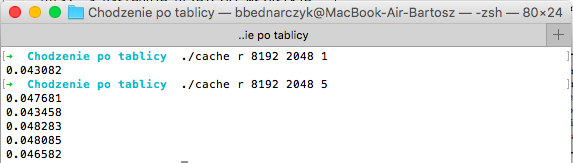
\includegraphics[scale=0.5]{zrzut_ekranu}
\end{figure}

\pagebreak

\subsection{Rozwiązanie}

Program czyta liczbę powtórzeń, wysokość oraz szerokość wiersza z polecenia. Następnie tworzy tablicę o podanym rozmiarze i wypełnia $(i ,j)$-tą komórkę wartością $i+j$. W kolejnym kroku przechodzi tablicę w zadanym kierunku zadaną liczbę razy, zapisując w każdej komórce tablicy wartość $1$ i podaje łączny czas przejścia. Wygenerowane przez program wyniki zostały uśrednione, a ich zestawienie prezentuję w poniższej tabeli:


\begin{table}[h!]
\centering
\label{my-label}
\begin{tabular}{|c|c|c|c|c|c|}
\hline
Wysokość tabeli & Szerokość tabeli & Liczba powtórzeń & Wynik R & Wynik C & Które lepsze? \\ \hline
32768 & 32768 & 10 & 17.0152810000 & 15.3259705000 & R \\ \hline
1024 & 4096 & 10000 &  0.0109929164 & 0.0902388145 & R \\ \hline
2048 & 2048 & 1000 &  0.0117144600 & 0.0963165690 & R \\ \hline
8192 & 2048 & 100 &  0.4078043900 & 0.0456573800 & R \\ \hline

\end{tabular}
\end{table}

Przez ,,R" i ,,C" będę oznaczał przejścia odpowiednio rzędami i kolumnami.

\subsection{Wnioski}

Patrząc na powyższą tabelę łatwo zauważyć, że przeglądanie tablicy rzędami jest efektywniejsze niż przejścia kolumnami. 
Wynika to z faktu, iż podczas pierwszego przejścia program wczytuje cały rząd do pamięci podręcznej, dzięki czemu przejścia między komórkami z tego samego rzędu są szybsze. Natomiast podczas przechodzenia tablicy kolumnami, program wczytuje pewien wiersz, a my przechodzimy do kolejnej kolumny (co powoduje wczytanie kolejnego wiersza), co pogarsza nasz wynik.
\end{document}